%%%%%%%%%%%%%%%%%%%%%%%%%%%%%%%%%%%%%%%%%%%%%%%%%%%%%%%%%%%%%%%%%%%%%%%%%%%%%%%%
%2345678901234567890123456789012345678901234567890123456789012345678901234567890
%        1         2         3         4         5         6         7         8

\documentclass[letterpaper, 10 pt, conference]{ieeeconf}  % Comment this line out
                                                          % if you need a4paper
%\documentclass[a4paper, 10pt, conference]{ieeeconf}      % Use this line for a4
                                                          % paper

\IEEEoverridecommandlockouts                              % This command is only
                                                          % needed if you want to
                                                          % use the \thanks command
\overrideIEEEmargins

\usepackage[cmex10]{amsmath}
%\usepackage[belowskip=-4pt, aboveskip=-0pt]{caption}
\usepackage{graphics} % for pdf, bitmapped graphics files
\usepackage{epsfig} % for postscript graphics files
\usepackage{epstopdf}
\usepackage{subfig}
\usepackage{mathptmx} % assumes new font selection scheme installed
\usepackage{times} % assumes new font selection scheme installed
\usepackage{amsmath} % assumes amsmath package installed
\usepackage{amssymb}  % assumes amsmath package installed
\usepackage{algorithmic}
\usepackage{array}
\usepackage{bm}
\usepackage{cite}
%\usepackage{natbib}
%\usepackage{titlesec}

\title{\LARGE \bf
{Vision guided learning based intelligent sewing system}
}

\author{Bidan Huang,
        Alessandro Vandini,
        Yang Hu,
        Guang-Zhong~Yang,~\IEEEmembership{Fellow,~IEEE}
\thanks{B. Huang, A. Vandini, Y. Hu and G.-Z. Yang are with the Hamlyn Centre for Robotic Surgery, Imperial College London, SW7 2AZ, London, UK (e-mail: b.huang@imperial.ac.uk). Bidan Huang and Yang Hu was supported by the EPSRC (EP/L020688/1).
}}

%\usepackage{caption}
%\setlength{\intextsep}{5pt plus 0pt minus 0pt}
\begin{document}

\maketitle
\thispagestyle{empty}
\pagestyle{empty}

%%%%%%%%%%%%%%%%%%%%%%%%%%%%%%%%%%%%%%%%%%%%%%%%%%%%%%%%%%%%%%%%%%%%%%%%%%%%%%%%
\begin{abstract}
This paper presents an intelligent sewing system for personalized stent graft manufacturing. Hand sewing is a challenging task for robotics, as it requires a high level dexterity and accuracy. Inspired by the medical suturing robots, we use a curved needle to achieve the task. We motorize a needle driver and attach it to a 7 d.o.f robot arm to manipulate the needle. Learning from demonstration approach is used to program the robot to sew the sent in the fabric. The demonstrated sewing skill is firstly segmented to several phases, and is encoded by statistical models. Robot sewing movements are generated from the models and are used for task execution. During the execution, a stereo vision system is adopted and guide the robot to adjust the learnt movement according to the needle pose. The system is implemented on a real robot system. We presents two experiments with this system and analyse the result experiment quantitatively. We show that our approach can robustly perform sewing with the same quality, as well as adapt to various needle pose.
\end{abstract}

%%%%%%%%%%%%%%%%%%%%%%%%%%%%%%%%%%%%%%%%%%%%%%%%%%%%%%%%%%%%%%%%%%%%%%%%%%%%%%%%


\section{Introduction}

%\begin{enumerate}
%\item{1} Bimanual manipulation-suturing is important and challenging
%\item{2} Our task is stent graft manufacturing
%%\item{3} Unsolved problems:Path planning,Adaptive to new context
%%\item{4} Our solutions:Vision + learn from demonstration,
%%Path planning - learning from demonstration, needle tracking, tool tracking,
%%Adaptive to new context - object centric approach + vision guided.
%\end{enumerate}
%~\cite{bidan2013grasp} 

A stent graft is a tubular structure composed of fabric supported by a metal mesh called a stent. It is widely used for a variety of conditions for endovascular intervention, but most commonly is used to reinforce an aneurysm.
Clinically, each stent graft needs to be customised to the patient anatomy, with fenestrations (openings) on the graft body to maintain the patency of important branches to vital organs. They often come at a significant cost in addition to long delays in manufacturing, largely due to the labour intensive manual tasks involved, subjecting patients to the risk of rupture during the waiting period and precluding treatment to patients presenting acutely. Improved manufacturing of personalised stentgrafts is therefore a critical unmet clinical demand and robot assisted manufacturing is being pursued.

This paper focus on the key process of the stentgraft manufacturing: sewing the stent to a fabric tube. The shape of the fabric tube is pre-designed for the patient anatomy and pre-manufactured. Unlike normal sewing, to sew the stent requires a ``3D sewing'' technology. Curved needles are commonly used for this task, as it can be pierced in and pierced out from one side of the fabric. We take a similar approach to robotize this task. 

Curved needle is widely used in surgery. Needle piercing is an important task for surgery robots. 

\section{System Overview}
Figure~\ref{fig:overview}

\subsection{Vision System}
Needle tracking / re-detection

\subsection{Learning from human demonstration}
Human demonstrate how to sew stent graft
Tracking needle (object centric approach)
Motion segmentation
Primitive motion learning

\subsection{Task execution}
Needle pose re-detection
Trajectory adaptation

\begin{figure}
\centering
{
\includegraphics[width=5cm]{./fig/overview.pdf}
\caption{\scriptsize{System overview of bimanual sewing robot}}

\label{fig:overview}
}
\end{figure} 
\section{Experiments}

\subsection{System setup}
The system is consisted of a robot mounted with a motorized needle driver, a robot mounted with a stent graft sewing mandrel, a fixed position needle driver, a curved needle and a stereo camera (Figure~\ref{}). The system workflow is as below:

\begin{enumerate}
\item{1}: Needle driver holding needle root
\item{2}: Vision system detect the needle pose relative to the needle driver
\item{3}: New robot trajectory is generated according to the needle pose
\item{4}: Needle driver approaching mandrel
\item{5}: Needle piercing into the fabric and the tip piercing out of fabric
\item{6}: Needle driver releasing the needle root, approaching the needle tip
\item{7}: Needle driver griping the needle tip and piercing the whole needle out of fabric
\item{8}: Needle driver bringing the needle to the second needle driver
\item{9}: The second needle driver griping the middle of the needle, the first needle driver griping the root of the needle
\end{enumerate}

% Stereo system
The stereo system is consisted of two identical Logitch HD cameras. The cameras are fixed on a tripod and are about 10$cm$ distance from each other. Stereo calibration and points triangulation are done by use the OpenCV. The calibration accuracy is measured by using the triangulation results to measure distance between two feature points on the camera view. The error is 0.89 $mm$.

The camera frame is registered to the robot frame by hand eye calibration. During the calibration, a key dot pattern is fixed on a know position of the robot end effector, whose origin is aligned with the end effector origin. The robot moves the key dots around and records the end key dot pattern positions in the robot frame, as well as in the camera frame. The rigid transformation between these two set of positions are computed by using the singular value decomposition technique. This transformation is hence the transformation from the robot frame to the camera frame. We mount the motorized needle driver on the end effector and register the tip pose to the robot. With the result of the hand eye calibration, the needle driver pose in the camera frame is computed.

The needle is initially grip at the very end of the needle driver and we assume that only small displacement of the needle pose will occur during the sewing task. The needle driver tip position is hence used as a prior of the needle position.

\subsection{Human demonstration}
For teaching robot the sewing task, we carry out four demonstrations. All demonstrations starts from the same position and sew the same slot on the mandrel. To control the quality of the stitches, across all demonstrations the needle pierces in at the same location and pierces out at the same location. At the beginning of each demonstration, the needle is placed at the same place and normal to the needle driver. Hence the needle pose in the robot frame can be computed accurately.

The demonstrations are segmented into three primitive movements, according to the needle drive open and close even. Figure~\ref{fig:segment} shows one segmentation results. Figure~\ref{fig:demo} shows the demonstrated needle driver trajectories in 3D.

\begin{figure}
\centering{
{\includegraphics[width=8cm]{./fig/seg_37.eps}}
\caption{\scriptsize{Segmentation result of human demonstration. The red, green and blue patches label the three segments of the motion}}
\label{fig:segment}
}\end{figure}


\begin{figure*}
\centering{
\subfloat[\scriptsize{Demonstrations of phase 1}] {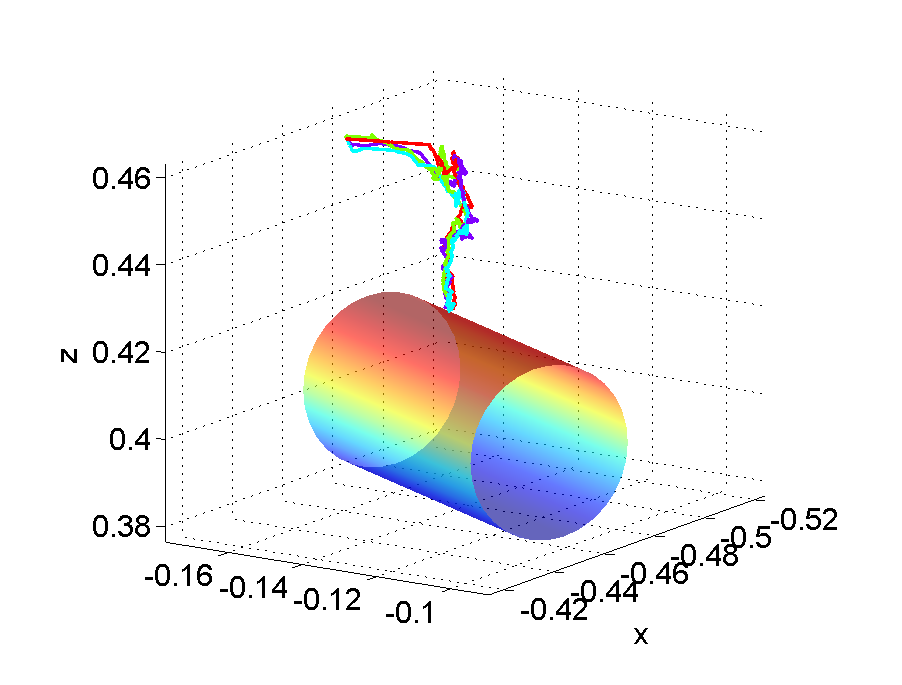
\includegraphics[width=8cm]{./fig/demo_1.eps}}
\subfloat[\scriptsize{Demonstrations of phase 2}]  {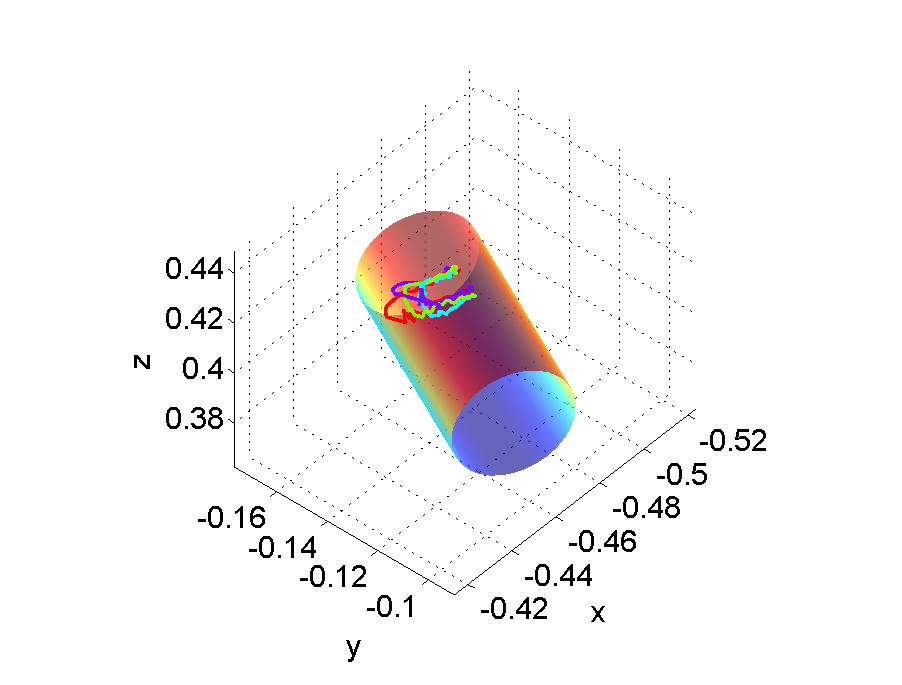
\includegraphics[width=8cm]{./fig/demo_2.eps}}
\\
\subfloat[\scriptsize{Demonstrations of phase 3}]  {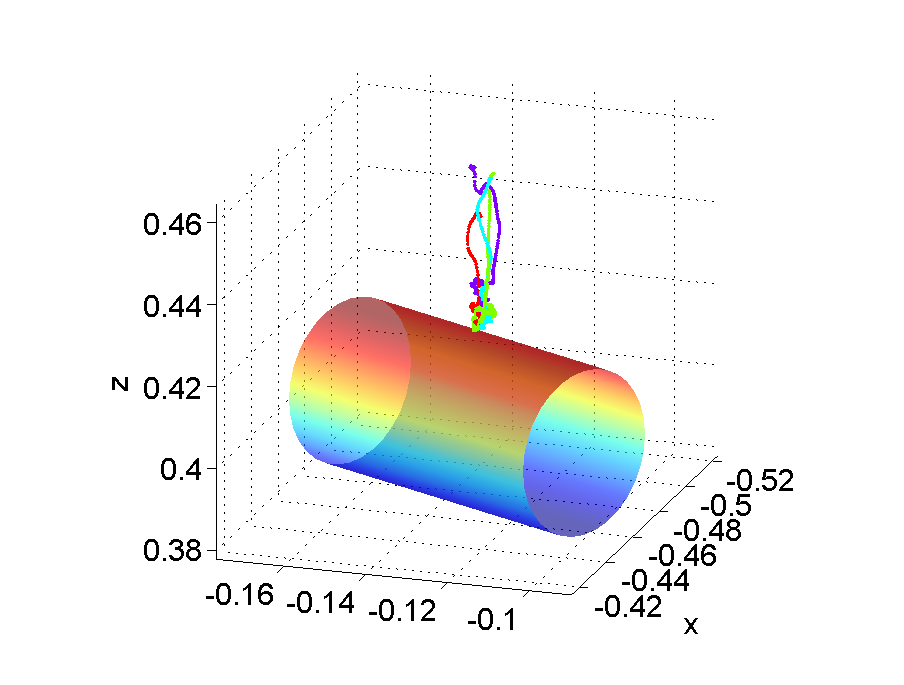
\includegraphics[width=8cm]{./fig/demo_3.eps}}
\subfloat[\scriptsize{Learnt trajectory of phase 1,2 and 3}]  {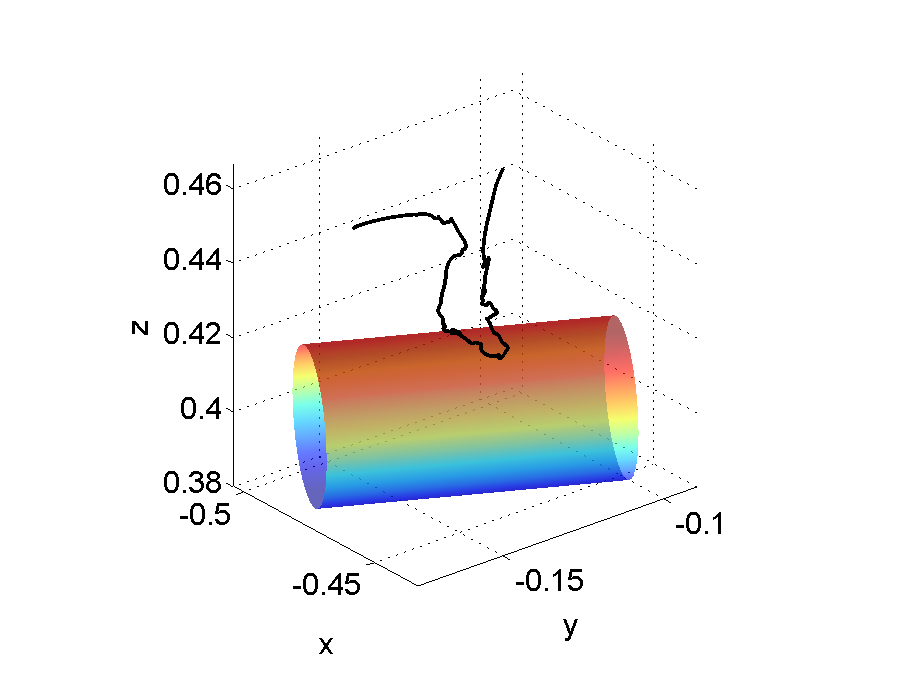
\includegraphics[width=8cm]{./fig/learn_123.eps}}
\caption{\scriptsize{Needle driver trajectories of human demonstrations and the learnt result. The cylinder represents the mandrel}}
\label{fig:demo}
}\end{figure*}

\subsection{Learning}
GMM is used to learn model for each phase. Figure~\ref{fig:GMR} shows a 2D projection of the build model of each phase. It can be seem from the model that the three phases have different charactoristics. Phase one has small variance from the beginning to the end, as all the movements start from the same point and pierce into the same location. The piercing movements are the same in order to produce similar stitches. Phase two has larger variance compare to phase one, as the needle is detached with the robot and the robot movement has less constraints. Phase three has small variance at the beginning, when the robot needs to pull out the needle from the same location, and has large variance once the needle is pulled out from the fabric. These show that the GMM can effectively capture the constraints at each phase and hence generate proper trajectories for the robot to complete the task.

\begin{figure*}
\centering{
\subfloat[\scriptsize{Phase 1}] {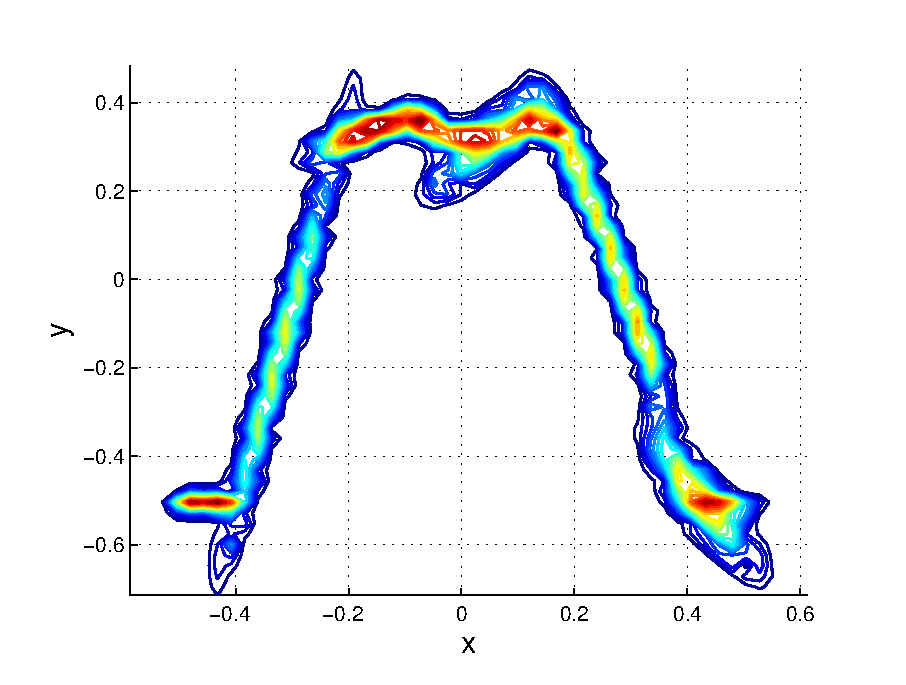
\includegraphics[width=6cm]{./fig/gmm_contour1_1-2.eps}}
\subfloat[\scriptsize{Phase 2}]  {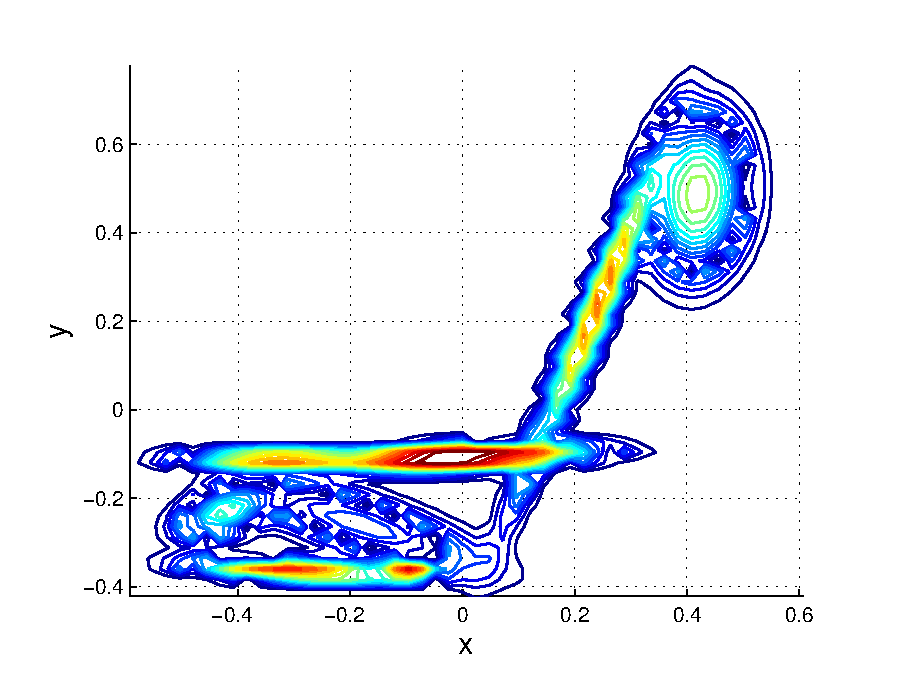
\includegraphics[width=6cm]{./fig/gmm_contour2_1-2.eps}}
\\
\subfloat[\scriptsize{Phase 3}]  {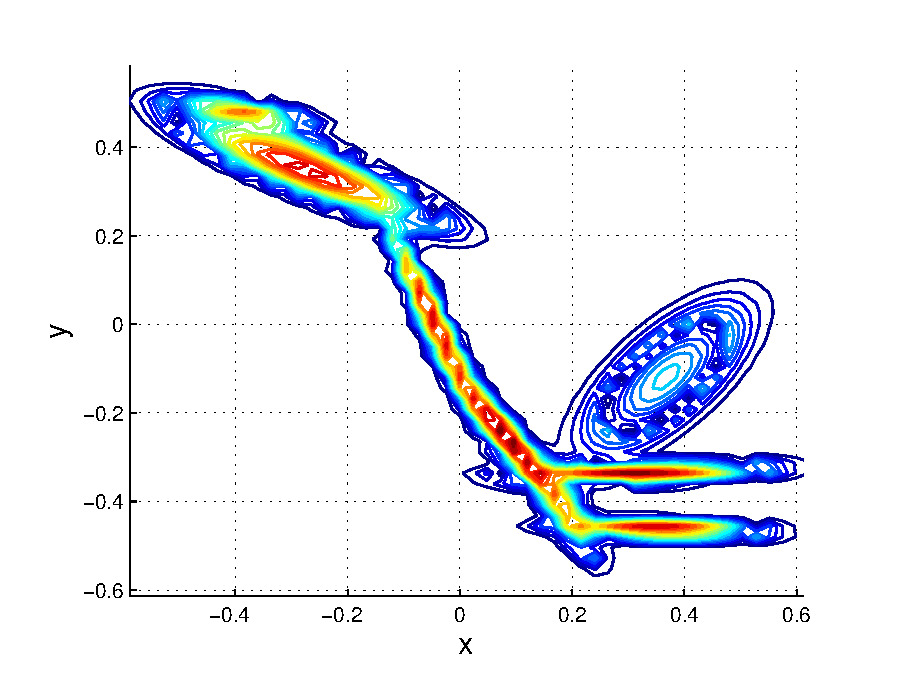
\includegraphics[width=6cm]{./fig/gmm_contour3_1-2.eps}}
\caption{\scriptsize{2D representation of the learnt models of different phases.}}
\label{fig:demo}
}\end{figure*}


\subsection{Task execution}

\section{Conclusion} 

In this paper a robotic system for sewing a stent graft is presented. We successfully teach the robot to sew with a curved needle as well as adapt to needle posture changes using a vision guidance system (needle posture re-detection). We analyse the robustness of our method quantitatively by two experiments: fabric piercing and needle regripping, which are the two critical parts for completing one sewing stitch. We show that our system is able to accomplish the sewing task effectively. Our vision system reconstructs the needle shape with sub-millimetres accuracy, and hence is able to guide robustly the robot to sew. The successful rate of our system is over 86$\%$. The failure case is due to the limited workspace caused by the robot joint limit. This problem can be leased by optimizing the task priority in the null space~\cite{yang2015}.

In this study, we use a single robot to manipulate the needle. The successful rate can be improved by using a second robot to cooperate the manipulation. This would make the tasks of both robot easier and also optimize each robot’s joint utilization. Our current system works as an open-loop manner for the needle adaptation part. Tracking the needle in real-time and implementing visual servoing algorithm is desired to increase the sewing accuracy. Further, the sewing presented is conducted in traditional way with needle drivers, in the future, customized sewing device will be designed by us to replace the needle holder to drive the needle performing fine movement. 

The system presented in this paper is a primary and promising study of robot hand sewing. Applications of the presented system and method are not limited only for stent graft sewing; it is also a promising technique for automating robotic suturing.



\bibliographystyle{plain}
\bibliography{ICRA16}


\end{document}
\end{document} 